\documentclass[tikz]{standalone}
\begin{document}

\tikzset{every picture/.style={line width=0.75pt}} %set default line width to 0.75pt        

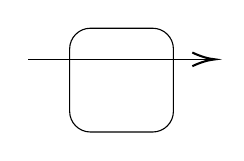
\begin{tikzpicture}[x=0.75pt,y=0.75pt,yscale=-1,xscale=1]
  %uncomment if require: \path (0,87); %set diagram left start at 0, and has height of 87

  %Rounded Rect [id:dp15569010121344817] 
  \draw (39.95,20) .. controls (39.95,14.48) and (44.43,10) .. (49.95,10) -- (79.95,10) .. controls (85.47,10) and
  (89.95,14.48) .. (89.95,20) -- (89.95,50) .. controls (89.95,55.52) and (85.47,60) .. (79.95,60) -- (49.95,60) ..
  controls (44.43,60) and (39.95,55.52) .. (39.95,50) -- cycle ;
  %Straight Lines [id:da5385679844937619] 
  \draw  (20,25) -- (108,25) ;
  \draw [shift={(110,25)}, rotate = 180] [color={rgb, 255:red, 0; green, 0; blue, 0 }  ][line width=0.75]
  (10.93,-3.29) .. controls (6.95,-1.4) and (3.31,-0.3) .. (0,0) .. controls (3.31,0.3) and (6.95,1.4) .. (10.93,3.29)
  ;

  % Text Node
  \draw (65,45) node   [align=left] {$\displaystyle \Ident$};

\end{tikzpicture}\end{document}
